\title{RADseq Works in Primates, Dammit.}
\author{
        Christina M. Bergey
			\and
			Luca Pozzi
			\and
			Todd R. Disotell
			\and
			Andrew S. Burrell
	}
\date{\today}

\documentclass[12pt]{article}

\usepackage{color}
\usepackage{graphics}

\begin{document}
\maketitle

\begin{abstract}
\ldots (This is the blurb from the email.) Our paper is an introduction to a 2nd generation sequencing technique for typing thousands of genome-wide markers from non-model organisms. Though it's been used in other taxa, this would be the first published application to primates. We demonstrate it with six Cercopithecoids and discuss its promise for doing mutli-locus population genetics in primates. \ldots
\end{abstract}

\section{Introduction}

During the first decades of molecular primatology, a formidable impediment to researchers was the need to develop and type polymorphic markers in a taxon of interest. The markers that resulted from this tedious and expensive task were often uninformative when applied outside of the population used in their design, necessitating further rounds of primer design or microsatellite assays, for example (Davey et al., 2011). Due to the bottleneck of marker discovery, many population genetic or phylogenetic studies in molecular primatology have been based on one or few loci (Ting and Sterner, published yet?). Such inferences can reliably give the evolutionary history of those particular regions of the genome, but they fail to adequately capture the complete complex history of the population given the mosaic nature of genomic evolution (some gene-tree species tree review ref). Adequate resolution depends on high marker density, and until recently that goal has been out of reach for many primate researchers.

The rapidly decreasing costs of DNA sequencing technology have promised revolutionary gains for primatology (Enard and Paabo 2004, maybe? Goodman et al 2005?). A primate researcher benefits from the many nearby sequenced and assembled reference genomes in the order, but genomic studies of non-model organisms nevertheless remain difficult. Though the cost of low coverage whole genome sequencing has fallen to a level feasible for many researchers' budgets, sequencing whole genomes for the tens or hundreds of individuals desired in a typical population genetic study is often prohibitively expensive and quite possibly superfluous. 

Fortunately, researchers have recently developed techniques that reduce the complexity of the genome and allow discovery and typing of thousands or tens of thousands of genome-wide makers in many individuals in a single step. RAD-seq is one such simple, inexpensive reduced representation technique which allows for the sequencing of small fragments of the genome adjacent to restriction enzyme cut sites (Baird et al., 2008). These RAD tags, or restriction-site association DNA tags, were originally developed for use in microarray hybridization typing (Miller et al., 2007), but an updated protocol substitutes second-generation DNA sequencing to rapidly discover and type SNPs (Baird et al., 2008). The lack of reliance on a reference genome and applicability to datasets of many individuals make it a promising technique for phylogenetic or population genetic studies in non-model organisms, such as many primates.

In the present study, we summarize the RAD-seq method in brief and note the many and varied applications since its development. We go on to discuss reasons that make RAD-seq promising for primatologists, and then demonstrate the technique in 5 primates: a lemur, New World monkey, Old World monkey, and two apes.  

\subsection{The RAD-seq Technique}

[The RAD-seq method, in brief. Also, Fig. 1]

\subsection{Previous RAD-seq Studies}

[Previous RADseq studies. Focus on pop gen, phylogeny studies]

\subsection{Prospective Primate Applications}

[Why it would be good in primates.]

Changing the restriction enzyme to a more or less frequent cutter allows fine grained control over the number of loci, number of individuals multiplexed, and depth of coverage, allowing researchers to tailor marker discovery to their hypothesis. 

\section{Methods}

\paragraph{Library Preparation and Sequencing}

	Genomic DNA from 5 primates was digested with \emph{PspXI} (New England Biolabs) and used to create a multiplexed RAD tag library. Our library preparation method followed that of Etter et al, 2011 with the following modifications: the P1 adapter top\textcolor{red}{(?)} oligonucleotide was modified to have an overhang corresponding to the cut site of \emph{PspXI}, and a longer P2 adapter suitable for paired end sequencing was used (P2\_top: 5'-\textcolor{red}{SEQUENCEHERE}-3'; P2\_bottom: 5'-\textcolor{red}{SEQUENCEHERE}-3'). Individual-specific barcodes contained in the P1 adapter differed by at least \textcolor{red}{three} nucleotides. We chose \emph{PspXI} based on the results of \emph{in silico} digestion of the human, rhesus macaque, and baboon reference genomes using custom Perl scripts (\textcolor{red}{refs}). We sequenced the prepared library as one 150-cycle paired-end run of an Illumina MiSeq at the NYU Langone Medical Center's Genome Technology Center using a spike-in of 30\% PhiX DNA to control for low diversity in the library at the barcode and restriction sites. Other individuals were sequenced alongside those of the present study. Sequences are available to download from the NCBI Short Read Archive (accession number \textcolor{red}{SRAXXXXXX.X}).

\paragraph{Sequence Analysis}

	Sequence reads were demultiplexed, or separated by barcode, and reads without an expected barcode or an intact restriction enzyme cut site were excluded from the analysis. Reads were then aligned to the rhesus macaque reference genome (v.1.0, Mmul\_051212/rheMac2, \textcolor{red}{ref}) using BWA with default parameters. Reads that were unmapped, unpaired, duplicates, or that had low mapping quality were removed after alignment using Picard (\textcolor{red}{ref}) and BamTools (\textcolor{red}{ref}). 

	After performing local realignment around indels with GATK (\textcolor{red}{ref}), SNPs and short indels were identified using SAMtools mpileup and BCFtools (\textcolor{red}{ref}). A minimum coverage of 3 reads and a maximum of 100 was required to call a SNP or an indel at a given location. Orthologous SNPs were tallied using VCFtools (\textcolor{red}{ref}).
	
	To assess how many restriction sites were successfully sequenced and to analyze the degree of overlap between multiplexed individual's datasets, we first found all possible \emph{PspXI} cut sites using the oligoMatch utility in the USCS Genome Browser program (\textcolor{red}{ref}). This allowed us to calculate the coverage of these restriction site-associated regions using BEDtools' multiBamCov program (\textcolor{red}{ref}).

\paragraph{Analysis Pipeline - Inferring Phylogeny}
\begin{itemize}
	\item Using method like cichlid people?
	\item Using method like Rubin et al? 
	\item Concatenated SNPs (not indels) into alignment. 
	\item Dimensions = 6 x ???
\end{itemize}

\section{Results}

% 3804227030 bp total (12,983,710 pairs of reads * (142bp + 151bp). This includes non-OWM taxa, remember.
% OWM sequencing reads: 6,125,860 total, half that many pairs
% Of those, 2029586 passed the filtration steps

6.1 million sequencing reads with an intact barcode and restriction enzyme cut site could be assigned confidently to one of the six Old World monkeys in the present study. Roughly 2.0 million of those reads were successfully mapped to the rhesus macaque genome and passed all quality control filtration steps. Relative to the reference genome, our study identified 531,175 SNPs and 24,260 small indels among all samples. Information for each individual is summarized in Table 1. 

\begin{table}[h]
\caption{Individual Sample Information}
\begin{center}
	\small
	\begin{tabular}{ p{3cm} || l || p{1.75cm} | p{1.75cm} || p{1.75cm} | p{1.75cm} | l }
		\hline
		Taxon & Source & \# Reads & \# Filtered Reads & \# Loci $\ge 1$ Read & \# Loci $\ge 3$ Reads & \# SNPs \\ \hline\hline
		\emph{Semnopithecus entellus} & \textcolor{red}{Unknown} & 1,367,050 & 306,248 & 47,516 & 24,052 & 363,501 \\ \hline
		\emph{Allenopithecus nigroviridis} & \textcolor{red}{Unknown} & 1,325,558 & 447,279 & 62,824 & 40,244 & 356,750 \\ \hline
		\emph{Macaca mulatta} & \textcolor{red}{Unknown} & 481,376 & 234,659 & 77,798 & 32,302 & 279,350 \\ \hline
		\emph{Cercocebus torquatus atys} & \textcolor{red}{Unknown} & 297,290 & 124,700 & 48,440 & 13,104 & 319,766 \\ \hline
		\emph{Papio anubis\textcolor{red}{?}} & \textcolor{red}{Unknown} & 743,556 & 313,676 & 74,582 & 39,062 & 316,118 \\ \hline
		\emph{Theropithecus gelada} & \textcolor{red}{Unknown} & 1,911,030 & 603,024 & 68,440 & 50,656 & 366,097 \\
		\hline
	\end{tabular}
\end{center}
\end{table}

In the rhesus macaque genome, we found 54,364 possible cut sites for \emph{PspXI} and 108,728 possible sequencing sites (two per cut site, one upstream and one downstream). Of those, 101,138 sites (93.02\%) were covered by at least one read in at least one individual, and for 13,456 sites (12.38\%), all six individuals had at least one read (Figure 1). When we restrict the analysis to sites with at least three reads, 80,448 sites (73.99\%) were covered in at least one individual and 1,354 sites (1.25\%) had all six individuals present.

\begin{itemize}
	\item Pairwise comparisons between individuals? Like X orthologous regions shared between Papio and Thero?
\end{itemize}

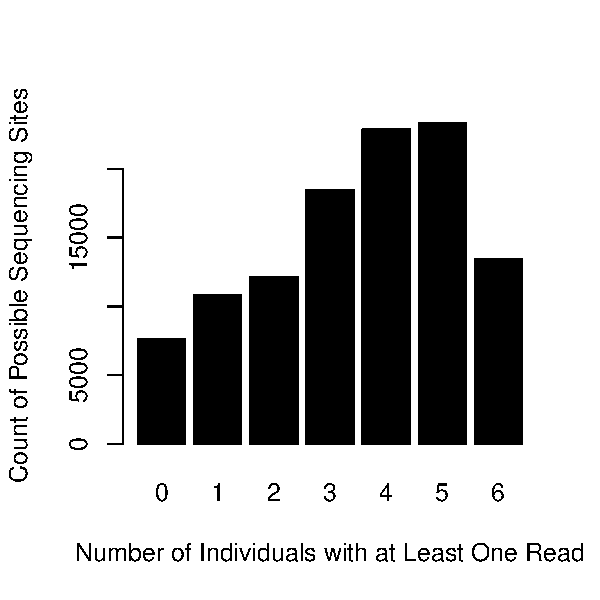
\includegraphics{figs/seq_site_coverage_by_ind}

\begin{itemize}
	\item SNP info from merged analysis
	\item SNP Venn diagram?
	\item Count orthologous SNPs shared between individuals. Pairwise?
\end{itemize}

\section{Discussion}
\begin{itemize}
	\item RADseq is viable tool for researcher interested in primate phylogenetics, pop. gen.
	\begin{itemize}
		\item Cheap and easy to create libraries. Competent lab can do it in two days. (Ha!)
		\item Multiplexing is great for pop gen studies.
		\item Enzyme choice allows control over coverage, number of individuals, number of loci.
		\item Baird: "different marker densities can be attained by choice of restriction enzyme"
	\end{itemize}
	\item Potential problems with RADseq method
	\item ddRADseq
	\item Promise for primatology
\end{itemize}

\section{Acknowledgements}
\begin{itemize}
	\item NYU Med School folk
	\item \textcolor{red}{Grants?}
\end{itemize}

\end{document}
